\subsection{Additional pipeline details}
\label{subsection:additional_pipeline_details}

\subsubsection{Data preprocessing}

\paragraph{Spike binning and unit selection.}
The Kilosort loader reads exported spike sample indices and cluster assignments, using a specified sampling rate, timebin duration, and recording interval. Spikes are counted in left-inclusive, right-exclusive timebins, retaining periods without spikes and preserving the correspondence between matrix columns and original cluster identifiers. Users may select units by identifier or cluster-quality label; no quality filtering is applied by default. Binning uses the exported acquisition timebase, while synchronization with behavioral measurements is handled separately.

\paragraph{Normalization.}
Activity can be z-scored or min--max scaled across timebins independently for each unit, or across units independently within each timebin. These operations serve different purposes: per-unit normalization adjusts differences in activity scale across units, whereas normalization within each timebin adjusts differences in activity scale across time.

\paragraph{Window construction.}
Consecutive timebins are grouped into windows of length $S$, with a configurable stride. When trial identifiers, session identifiers, timestamps, and validity masks are supplied, windows crossing corresponding boundaries, temporal gaps, or invalid observations are excluded. Restricting eligible timebins to a data partition also helps prevent windows from crossing training, validation, and test boundaries. For paired input and target windows, these restrictions apply to both windows; their pairing is defined before batching.

\subsubsection{Model training}
\label{subsubsection:model_architecture_training}

We use $S$ and $N$ for the input window length and unit count, $D$ latent dimensions, $B$ examples per batch, and training sparsity parameter $k$. The subscript $\mathrm{out}$ denotes target dimensions, allowing both window length and unit count to differ from the input in the transcoder case. The dataset defines batch pairs of inputs $\mathbf{Y}\in\mathbb{R}^{B\times S\times N}$ with targets $\mathbf{\Psi}\in\mathbb{R}^{B\times S_{\mathrm{out}}\times N_{\mathrm{out}}}$; the prediction $\hat{\mathbf{\Psi}}$ has the target's shape. Autoencoding is the special case $\mathbf{\Psi}=\mathbf{Y}$, with $S_{\mathrm{out}}=S$ and $N_{\mathrm{out}}=N$. ``Overcompleteness'' implies $D>N$.

\paragraph{Window SEDs.}
The FW-SED encoder vectorizes the full $S\times N$ window and applies one learned linear projection to produce $D$ latent pre-activations. This is the most direct temporal extension of a conventional SED: a hidden layer neuron (latent) can assign a different weight to every unit--timebin pair and can therefore represent a motif at a particular position within the window. 

The TW-SED encoder treats the $N$-dimensional population activity at each of the $S$ input timebins as one token, projects it into an embedding space, adds learned absolute-position embeddings, and applies one or more self-attention blocks. The representation at the final token is then projected to the same $D$ latent pre-activations. Causal attention restricts this readout to the present and preceding bins.

In preliminary TW-SED experiments, we also tried concatenating the contextualized outputs from all tokens and projecting this full-window representation into latent pre-activations. This yielded worse recovery of ground-truth latents than projecting only the contextualized final token, motivating the latter readout.

For either Window encoder, ReLU produces nonnegative latent activations, and BatchTopK enforces latent sparsification. The decoder applies a learned linear mapping and bias to the sparse activations, followed by an activation function $g$, to predict the full target window $\hat{\mathbf{\Psi}}\in\mathbb{R}^{B\times S_{\mathrm{out}}\times N_{\mathrm{out}}}$ jointly. $g$ can be the identity function, ReLU, or softplus: identity output permits signed reconstructions, useful for z-scored activity, whereas ReLU or softplus enforces nonnegativity, for spike counts outputs, for example. The decoder weights specify each latent's contribution to output units at each timebin within the target window before the output activation, making the learned spatiotemporal patterns explicit.

\paragraph{Training objective and algorithm.}
For $L$ nested Matryoshka levels, $D_\ell$, $k_\ell$, and $\lambda_\ell$ denote the dictionary width, sparsity parameter, and reconstruction-loss weight of level $\ell$, with $D_L=D$. A single-level SED has $L=1$, $D_1=D$, and $k_1=k$. At each Matryoshka level $\ell$, BatchTopK retains the $Bk_\ell$ largest activations across the batch, considering only that level's $D_\ell$ latent dimensions. Each level attempts to reconstruct the complete target using the time-weighted loss,
\begin{equation}
\label{eq:time_weighted_reconstruction_loss}
    \mathcal{L}_{w}(\mathbf{\Psi},\hat{\mathbf{\Psi}})
    = \frac{\sum_{s=1}^{S_{\mathrm{out}}} w_s\,\mathcal{E}(\hat{\mathbf{\Psi}}_{:,s,:},\mathbf{\Psi}_{:,s,:})}
           {\sum_{s=1}^{S_{\mathrm{out}}} w_s},
\end{equation}
where \hyperref[paragraph:reconstruction_loss_functions]{$\mathcal{E}$} denotes the chosen elementwise reconstruction loss (e.g., \metric{MSE}), averaged over examples and output units at each target timebin, with one positive weight $w_s$ per target timebin. Reconstruction metrics may be reported separately for each timebin within the target window.

\hyperref[algorithm:sed_model_training]{Algorithm 1} specifies one training step. The encoder $E_\theta$ is the single-bin, flat-window, or transformer-window encoder; the reconstruction indices $s=1,\ldots,S_{\mathrm{out}}$ and $n=1,\ldots,N_{\mathrm{out}}$ refer to target timebins and output units. The shift-equivariant variant uses time-indexed latent occurrences and a convolutional decoder, as described below.

\begin{algorithm}[h]
\caption{Training step with one latent vector per input window}
\label{algorithm:sed_model_training}
\begin{algorithmic}[1]
\Require Input $\mathbf{Y}\in\mathbb{R}^{B\times S\times N}$; target $\mathbf{\Psi}\in\mathbb{R}^{B\times S_{\mathrm{out}}\times N_{\mathrm{out}}}$
\Require Encoder $E_\theta$; decoder $\mathbf{W}_{\mathrm{dec}}\in\mathbb{R}^{S_{\mathrm{out}}\times N_{\mathrm{out}}\times D}$
\Require Decoder bias $\mathbf{b}_{\mathrm{dec}}\in\mathbb{R}^{S_{\mathrm{out}}\times N_{\mathrm{out}}}$ and output activation $g$
\Require Levels $\{D_\ell,k_\ell,\lambda_\ell\}_{\ell=1}^{L}$, time weights $w_s>0$, auxiliary weight $\gamma$
\Procedure{TrainStep}{$\mathbf{Y},\mathbf{\Psi}$}
    \State $\mathbf{Z}\gets\operatorname{ReLU}(E_\theta(\mathbf{Y}))\in\mathbb{R}^{B\times D}$
    \State $\mathcal{L}_{\mathrm{recon}}\gets0$
    \For{$\ell=1,\ldots,L$}
        \State $\tilde{\mathbf{Z}}_\ell\gets\operatorname{BatchTopK}(\mathbf{Z}_{:,1:D_\ell},Bk_\ell)$
        \State $\hat{\mathbf{\Psi}}_{\ell,b,s,n}\gets g\!\left(\sum_{j=1}^{D_\ell}\tilde Z_{\ell,b,j}W_{\mathrm{dec},s,n,j}+b_{\mathrm{dec},s,n}\right)$
        \State $\mathcal{L}_{\mathrm{recon}}\gets\mathcal{L}_{\mathrm{recon}}+\lambda_\ell\mathcal{L}_{w}(\mathbf{\Psi},\hat{\mathbf{\Psi}}_\ell)$
    \EndFor
    \State $\mathcal{D}_{\mathrm{dead}}\gets\operatorname{InactiveLatents}(\text{activation history})$
    \State $\mathbf{R}\gets\mathbf{\Psi}-\operatorname{stopgrad}(\hat{\mathbf{\Psi}}_L)$
    \State $\mathcal{L}_{\mathrm{aux}}\gets\operatorname{DeadLatentResidualLoss}(\mathbf{Z},\mathbf{R},\mathcal{D}_{\mathrm{dead}})$
    \State $\mathcal{L}_{\mathrm{total}}\gets\mathcal{L}_{\mathrm{recon}}+\gamma\mathcal{L}_{\mathrm{aux}}$
    \State Backpropagate $\mathcal{L}_{\mathrm{total}}$; project decoder gradients tangent to unit-norm dictionary
    \State Update parameters; normalize decoder atoms; update latent inactivity counters
\EndProcedure
\end{algorithmic}
\end{algorithm}

\paragraph{Reconstruction loss functions.}
\label{paragraph:reconstruction_loss_functions}
For a fixed target timebin $s$, let $\psi=\Psi_{b,s,n}$ and $\hat{\psi}=\hat{\Psi}_{b,s,n}$ denote target and reconstruction entries, and let $\langle\cdot\rangle_{b,n}$ denote the mean over examples and output units. Three loss functions are mean squared error (MSE), mean squared log error (MSLE), and Poisson KL divergence (PKL):
\begin{align}
\mathcal{E}_{\mathrm{MSE}} &= \left\langle(\hat{\psi}-\psi)^2\right\rangle_{b,n},\\
\mathcal{E}_{\mathrm{MSLE}} &= \left\langle\bigl[\log(1+\psi)-\tau\log(1+\max(\hat{\psi},0))\bigr]^2\right\rangle_{b,n},\\
\mathcal{E}_{\mathrm{PKL},\epsilon} &= \left\langle(\psi+\epsilon)\log\!\frac{\psi+\epsilon}{\hat{\psi}+\epsilon}+\hat{\psi}-\psi\right\rangle_{b,n}.
\end{align}
The MSLE expression follows the implementation's clipping of negative reconstructions and requires $\psi>-1$. Setting $\tau=1$ gives the usual squared log error. For nonnegative targets, $\tau>1$ more heavily penalizes overestimation, whereas $0<\tau<1$ more heavily penalizes underestimation. The preliminary PKL implementation used nonnegative targets and reconstructions, adding $\epsilon>0$ to both to avoid evaluating logarithms at zero (default $10^{-6}$).

In preliminary comparisons with all other settings held fixed, MSLE yields better reconstruction fidelity and recovery of synthetic ground-truth features for raw spike counts, whereas we observe no performance difference between MSE and MSLE for standardized spike data. For MSLE, setting $\tau=1$ generally gives the best results among the tested values. PKL performs worse than MSE and MSLE in these experiments, and choosing the offset $\epsilon$ introduces an additional numerical consideration near zero. The synthetic spatial models in \autoref{figure:synthetic_results}c,d use MSLE with $\tau=1$; all other reported NLDisco models in the synthetic, Churchland, and Aeon results use MSE.

\paragraph{Dead-latent auxiliary loss.}
Some latents stop activating during training and therefore contribute nothing to reconstruction (marked in $\mathcal{D}_{\mathrm{dead}}$). To encourage their reuse, we  train them to fit the residual error $\mathbf{R}$ left by the highest Matryoshka level, similar to the AuxK loss of~\citet{gao_2025_topk_saes}. This auxiliary loss encourages reuse through gradient updates without explicitly reinitializing inactive latents. This auxiliary branch selects activations only from these dead latents using BatchTopK, with a separate sparsity budget determined by their number and a configured fraction of the dictionary width. This keeps the auxiliary reconstruction sparse, encouraging a small set of dead latents to explain the residual rather than distributing it across many weakly activated features, ostensibly improving interpretability. The residual is treated as a fixed per-batch target during backpropagation for these dead latents only. When no latents are dead, the auxiliary loss is zero.

\paragraph{Optional shift-equivariant mode.}
The TW-SED's shift-equivariant configuration changes the scientific interpretation from a feature tied to one window alignment to a motif that can occur at different positions within the window. Absolute-position embeddings are removed, and learned relative-position biases encode offsets between timebins, allowing the same detector to operate at every timebin. Rather than reducing the transformer sequence to its final token, the latent projection produces a temporally indexed activation tensor in $\mathbb{R}^{B\times S\times D}$. Batch top-$k$ is then applied across valid time--latent occurrences, so the same latent may activate at different positions in different windows. This can remove obfuscation from the same feature being captured by different latents at different positions within the window.

This mode uses aligned input and target windows on a shared time grid, with $S_{\mathrm{out}}=S$. The corresponding decoder replaces the fixed full-window linear dictionary with a transposed temporal convolution. Each latent has a motif kernel specifying its contribution to each output unit at temporal offsets relative to the motif's activation bin. Every sparse occurrence places a shifted copy of that kernel into the reconstruction. Causal kernels reconstruct the occurrence and preceding support; centered kernels reconstruct symmetrically around it. Because unequal timebin weights would privilege absolute positions and break the intended symmetry, this mode requires all $w_s$ to be equal.

\paragraph{Hyperparameter guidance.}
\label{paragraph:hyperparameter_sweeps}
\label{subsubsection:hyperparameter_sweeps}
NLDisco uses Hydra-based YAML configurations and command-line overrides to specify data, architecture, and optimization settings. Automated sweeps run on CPUs or GPUs using local search or Weights \& Biases, with local execution or Slurm scheduling through Submitit.

We recommend jointly varying dictionary width $D$ and sparsity $k$, testing several sparsity levels at each width rather than automatically holding $k/D$ fixed. For recordings similar to those studied here, $D\in\{128,192,256\}$ provides a practical starting range based on our experiments; dictionary width is not determined solely by the number of recorded units or windows. Vary $k$ separately: our synthetic experiments use average budgets as small as $k=4$, whereas real-data configurations explore larger budgets. The appropriate choices also depend on window duration, preprocessing, and the diversity and frequency of the features to be recovered. Comparisons should hold preprocessing, bin width, window lengths, batch size, and evaluation observations fixed unless explicitly varied. Assess reconstruction fidelity alongside measured mean \metric{L0}, redundant latents, dead latents, and consistency of recovered features across training seeds (see ~\hyperref[subsubsection:model_evaluation_details]{\ref*{subsubsection:model_evaluation_details}}, ~\hyperref[subsubsection:latents_evaluation_details]{\ref*{subsubsection:latents_evaluation_details}} for examples). Larger dictionaries offer more candidates when searching for the best latent; report the search width and any controls for candidate count. Neither the largest dictionary nor the lowest reconstruction error is necessarily preferred.

For training optimization, we use Adam with no weight decay, an initial learning-rate setting of $0.005$, $(\beta_1,\beta_2)=(0.9,0.999)$, and $\epsilon=10^{-8}$. We do not find additional weight regularization, such as AdamW's decoupled weight decay, necessary in these experiments, where BatchTopK constrains latent activity and the decoder weights are normalized. Exploratory comparisons with NAdam do not yield a clear improvement over Adam. All of our experiments in this paper use the same learning rate schedule, defined as fractions of the total number of optimization steps: linear warmup over the first 10\%, a constant learning rate until 50\%, and a single cosine decay toward 1\% of the initial rate over the remaining updates. This schedule depends on update count rather than reconstruction loss, so short-term loss fluctuations do not trigger learning-rate reductions. Batch sizes of 256--1,024 windows are used in our experiments. For new datasets, a small learning-rate sweep around the initial setting can be useful.

When monitoring training, it can be useful to distinguish three broad phases: 1) initial representation learning, when latents capture general structure; 2) specialization, when individual latents develop more distinct activation patterns; and 3) refinement, when those patterns undergo smaller adjustments. These phases are a qualitative guide rather than fixed stages that every run must exhibit.

\subsubsection{Model evaluation}
\label{subsubsection:model_evaluation_details}

Model evaluation considers reconstruction fidelity, dictionary width $D$, and activation sparsity $k$ separately. NLDisco reviews dictionary quality via latent sparsity metrics (\autoref{figure:model_eval} top). The \metric{L0} norm measures the number of active latents in an example, set indirectly by the batch top-$k$ parameter, while the latent activation density visualizes the distribution of activation frequencies across latents. Together these metrics reveal whether the model has learned a code that uses many latents efficiently while avoiding common pitfalls such as ``representational collapse'' into too many constantly active latents and widespread ``feature death'' in which a large portion of the dictionary never activates. These sparsity metrics are complemented by a couple of reconstruction fidelity metrics: variance explained (\metric{R^2}) and cosine similarity of reconstruction-to-target neural activity across target units and timebins (\autoref{figure:model_eval} bottom). High scores indicate faithful reconstruction under these metrics. Importantly, more available latents $D$ or more active latents $k$ can improve reconstruction, but reconstruction alone does not establish latent interpretability: if the neural code is segmented across too many or too few latents, the resulting features may be difficult to interpret.

\begin{figure}[th]
    \centering
    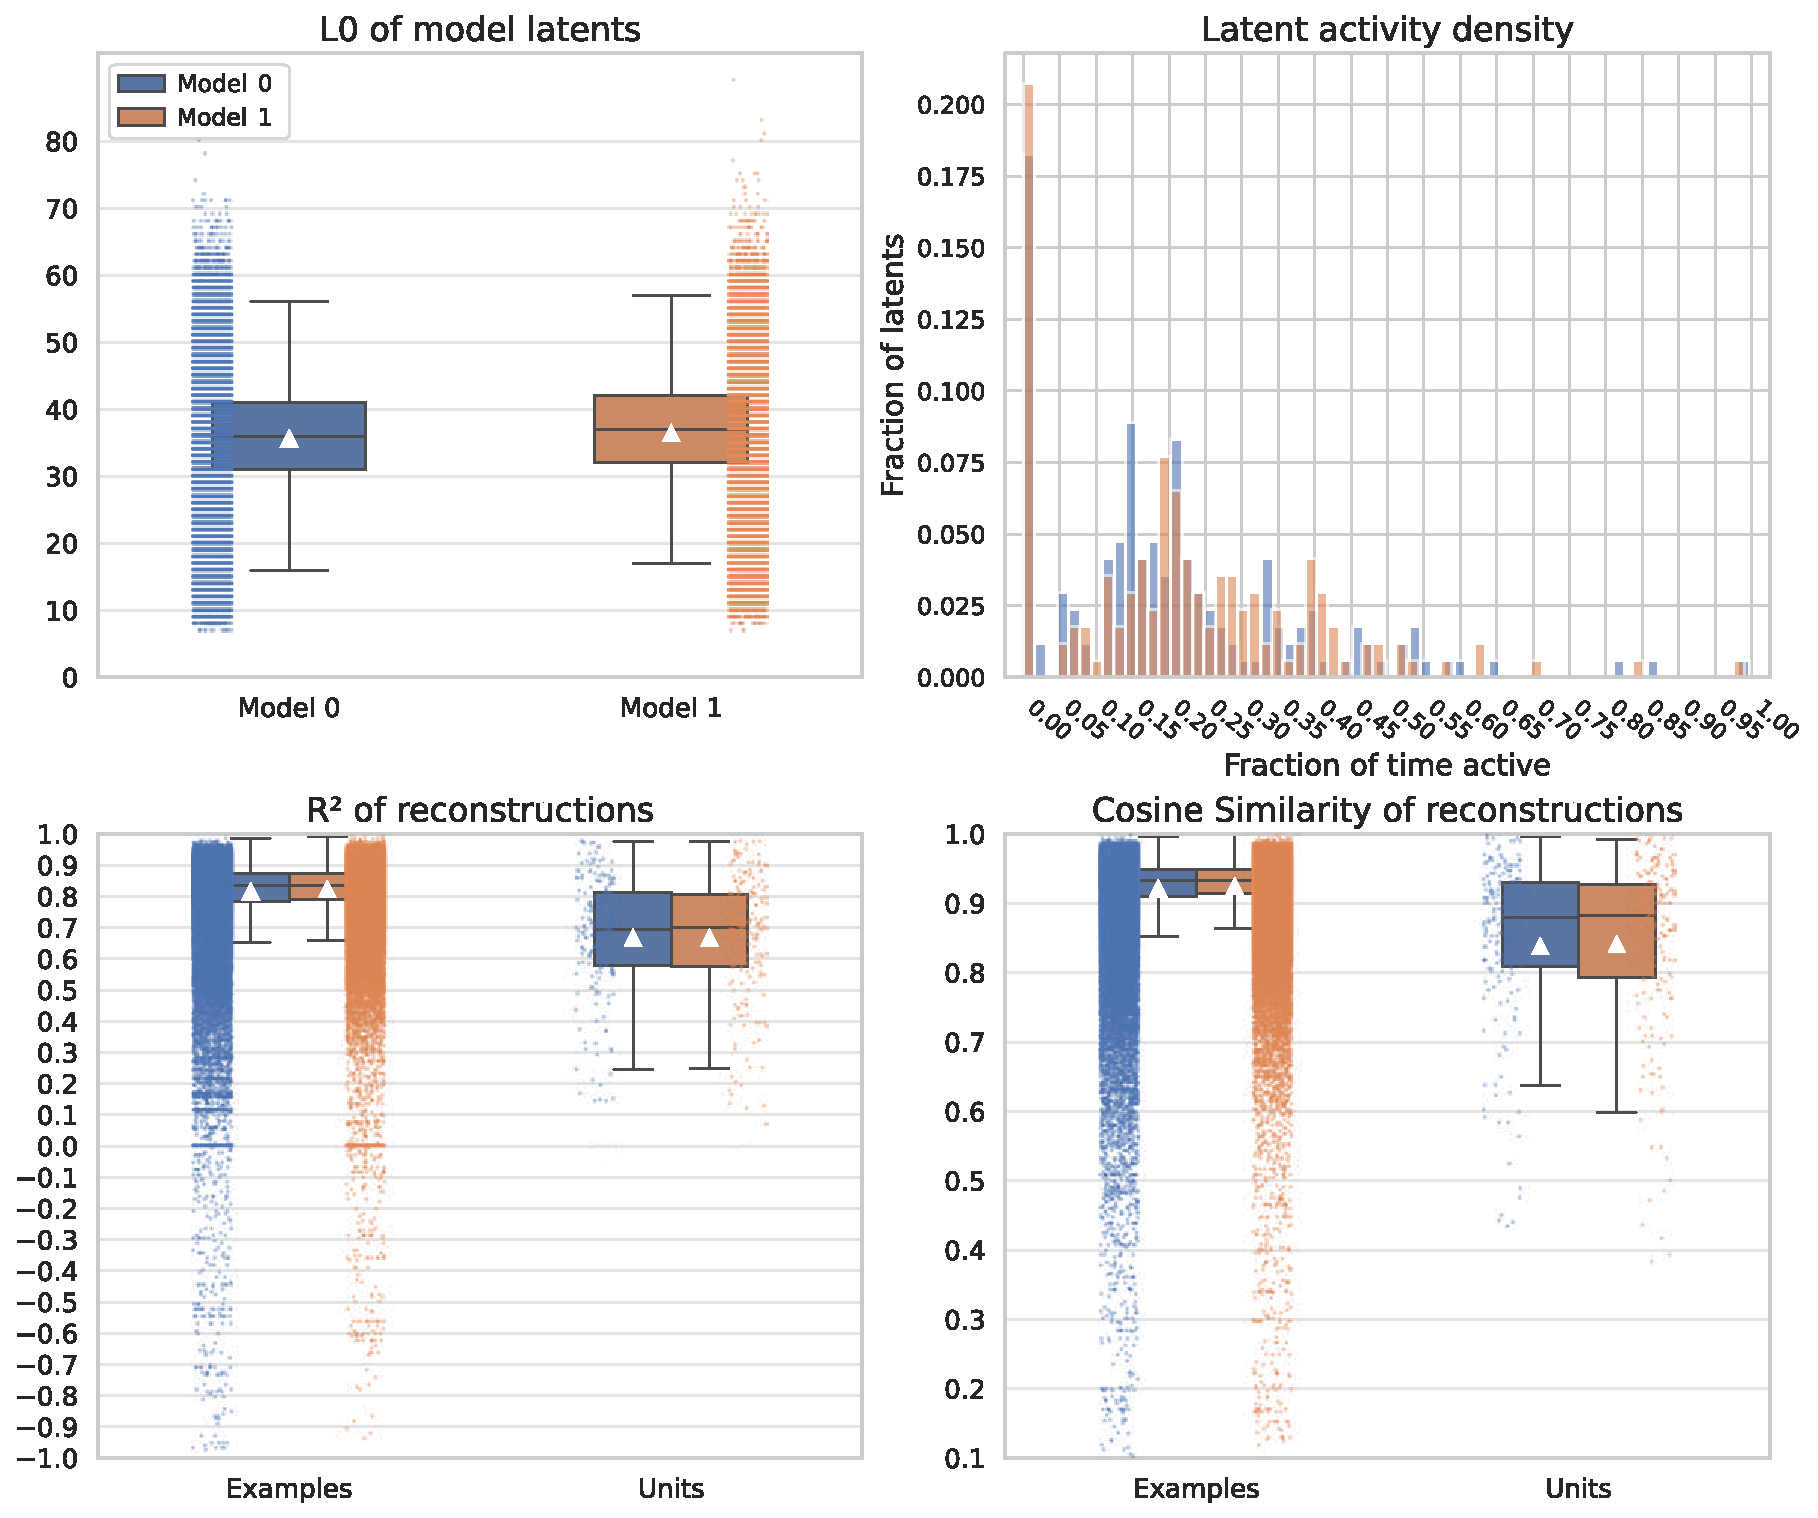
\includegraphics[width=\linewidth]{figures/model_eval.pdf}
    \caption{
        \textbf{Model evaluation metrics.} \\
        \small This example uses Allen Institute Visual Coding Neuropixels data~\citep{siegle_2021_allen_datasets}. The SED model has $L=3$ nested Matryoshka levels with $(D_1,k_1)=(128,12)$, $(D_2,k_2)=(224,24)$, and $(D_3,k_3)=(320,36)$, and $B=1024$ examples per batch. Each level selects $Bk_\ell$ activation entries across the batch from its first $D_\ell$ latents. The recording contains $N=200$ units, and the model is trained on 182,868 single-bin examples ($S=1$) of 50-ms spike counts. The model exhibits an approximately normal distribution of the latent \metric{L0} norm, few dead or tonically active latents, and high neural reconstruction fidelity as measured by \metric{R^2} and cosine similarity across both units and examples, all indicators of healthy training.
    }
    \label{figure:model_eval}
\end{figure}

Two optional diagnostics examine how individual latents support reconstruction and how well reconstruction preserves frequency content. 

\textit{Latent ablation importance} measures the change in reconstruction error when one latent's activations are set to zero, holding all other activations fixed. We report the increase in mean-squared error and its variance-normalized counterpart, $\Delta R_j^2=(\mathrm{SSE}_{-j}-\mathrm{SSE}_{\mathrm{full}})/\mathrm{SST}$, where $\mathrm{SST}$ centers each target unit at each lag across evaluation windows. Importantly, these scores are not additive shares of explained variance, and unequal contributions need not indicate a problem: meaningful features may differ in prevalence and strength.

\textit{Spectral reconstruction fidelity} compares each unit's target and reconstructed power spectral densities using Welch's method, with a specified bin duration and spectral segment duration. We assemble one reconstruction per physical timebin at a fixed position within the target window (its endpoint by default), and process contiguous stretches separately. Outputs include the spectra, integrated absolute spectral differences normalized by target power, and optional frequency-band power differences. Spectra are computed in the same normalized units as the targets; zero target power makes relative errors undefined. Matching spectra supports preservation of frequency content, but does not establish preservation of phase or event timing.

\subsubsection{Latents evaluation}
\label{subsubsection:latents_evaluation_details}

\paragraph{Visualization and interpretation.}
In general, we recommend building a simple dashboard or set of linked plots that places latent activations alongside behavioral and environmental variables: inspect tuning curves and activating examples to develop candidate feature descriptions, then assess these descriptions across the full eligible population, including examples in which the latent is inactive.

In this paper, we evaluate latents using dataset-specific visualizations. In \hyperref[subsection:synthetic_results]{\ref*{subsection:synthetic_results}} we compare spatial tuning and activating trajectories with known place fields and movement directions, in \hyperref[subsection:churchland_results]{\ref*{subsection:churchland_results}} we examine latent activity alongside movement kinematics and trial conditions, and in \hyperref[subsection:aeon_results]{\ref*{subsection:aeon_results}} we examine latent activity during spontaneous foraging, including wheel activity and movement around the patch. These observations inform candidate feature descriptions, which we quantify over explicitly defined comparison populations using the shared metrics described below.

\paragraph{Coverage, specificity, selectivity, and discriminability.}
\label{subsection:selectivity_score}
To assess a candidate feature, we need to measure both how often a latent detects its proposed condition and how often it activates outside that condition. Coverage and specificity describe these two aspects, selectivity summarizes the relative preference, and discriminability measures how well activation values separate these two aspects across thresholds.

Let $A_l$ denote the event that latent $l$ is active under the stated activation rule, and let $C$ denote a behavioral or environmental condition, such as speed in a specified interval. The true-positive rate (\metric{TPR}) measures how often the latent is active when the condition holds; the false-positive rate (\metric{FPR}) measures how often it is active otherwise. Coverage (\metric{Cov}) = \metric{TPR}, specificity (\metric{Spec}) = $1 - \metric{FPR}$, and selectivity (\metric{Sel}) compares the two activation probabilities (estimated as fractions of eligible examples in each condition class):
\begin{align}
\metric{TPR}_l(C) &= P(A_l\mid C),\notag\\
\metric{FPR}_l(C) &= P(A_l\mid\neg C),\notag\\
\metric{Cov}_l(C) &= \metric{TPR}_l(C),\label{eq:latent_coverage}\\
\metric{Spec}_l(C) &= 1-\metric{FPR}_l(C),\label{eq:latent_specificity}\\
\metric{Sel}_l(C) &= \frac{\metric{TPR}_l(C)}{\metric{TPR}_l(C)+\metric{FPR}_l(C)}.\label{eq:latent_selectivity}
\end{align}

Selectivity should be read alongside coverage. For example, $\metric{TPR}=0.10$, $\metric{FPR}=0.01$ and $\metric{TPR}=0.90$, $\metric{FPR}=0.09$ both give $\metric{Sel}\simeq0.909$, despite very different coverage. A highly selective latent may therefore detect only a small subset of a condition's occurrences.

\label{paragraph:latent_discrimination}
To quantify discriminability across activation thresholds, we use the area under the receiver operating characteristic curve (\metric{AUROC}), which measures how reliably condition-positive examples have higher latent activity than condition-negative examples:
\begin{equation}
\label{eq:latent_auroc}
\metric{AUROC}=P(z_C>z_{\neg C})+\tfrac12P(z_C=z_{\neg C}),
\end{equation}
where $z_C$ and $z_{\neg C}$ denote the same latent's activation value for an example drawn from inside and outside condition $C$, respectively. Each comparison counts as correct when the positive example has the larger activation, incorrect when it has the smaller activation, and half-correct when the activations are equal.

\paragraph{Decoding.}
\label{paragraph:latent_decoding}
We also assess how well a feature can be classified as present ($y = 1$) or absent ($y = 0$) based on latent activity by fitting an $\ell_2$-regularized logistic-regression decoder,
\begin{equation}
\label{eq:latent_logistic_decoder}
\widehat P(y=1\mid\mathbf z)=\sigma\!\left(b+\mathbf w^\top\widetilde{\mathbf z}\right),
\qquad \sigma(a)=\frac{1}{1+\exp(-a)},
\end{equation}
where $\widetilde{\mathbf{z}}$ is standardized $\mathbf{z}$ latent activations, $\mathbf w$ the learned regression weight, and $b$ an intercept term. A single-latent decoder uses a scalar $w$ to weight the specified latent; a full-space decoder uses a vector $w$ to weight all latents in the LVM.


We fit the decoder by minimizing binary cross-entropy with an $\ell_2$ penalty on its weights:
\begin{equation}
\label{eq:latent_decoder_loss}
\begin{aligned}
\mathcal L_{\mathrm{dec}}(\mathbf w,b)
&= -\sum_{i=1}^{M}\left[y_i\log\widehat p_i+(1-y_i)\log(1-\widehat p_i)\right]
+\frac{\lambda_{\mathrm{dec}}}{2}\|\mathbf w\|_2^2,\\
\widehat p_i &= \sigma\!\left(b+\mathbf w^\top\widetilde{\mathbf z}_i\right).
\end{aligned}
\end{equation}
Here, $M$ is the number of training examples, $y_i$ indicates whether the behavioral condition holds, and $\lambda_{\mathrm{dec}}$ controls regularization strength, which we select from \(\lambda_{\mathrm{dec}}\in\{10^{-3},10^{-2},10^{-1},1,10,100,1000\}\) to maximize validation set \(\metric{AUROC}\). We optimize the decoder weights and intercept using L-BFGS over the full training set, with a convergence tolerance of $10^{-5}$ and a maximum of 1,000 iterations per fit.

The reported \metric{Decode} score is test balanced accuracy: the average fraction of condition-positive examples predicted positive and condition-negative examples predicted negative,
\begin{equation}
\label{eq:latent_decode_balanced_accuracy}
\metric{Decode}=\tfrac12\bigl(\metric{TPR}_{\mathrm{decoder}}+1-\metric{FPR}_{\mathrm{decoder}}\bigr).
\end{equation}

This gives both classes equal weight, with 0.5 for a constant prediction and 1 for perfect classification. For each fitted decoder, we select a single probability threshold $t$ that maximizes balanced accuracy on the validation set. An example is classified as condition-positive when its predicted probability $\widehat P(y=1\mid\mathbf z)\ge t$, and condition-negative otherwise. The decoder weights and this threshold are then held fixed for all test examples. 

\paragraph{Source activity traceback.}
\label{paragraph:source_activity_traceback}

To identify which recorded units and timebins contribute to a latent's activation, we trace its response back through the encoder. For an input window $\mathbf{Y}$, let $h_l(\mathbf{Y})$ denote latent $l$'s pre-activation, before ReLU and sparsification. We assign each input entry the attribution score:

\begin{equation}
\label{eq:source_activity_traceback}
a_{l,s,n}(\mathbf{Y})=Y_{s,n}\,\frac{\partial h_l(\mathbf{Y})}{\partial Y_{s,n}}.
\end{equation}

Here, $Y_{s,n}$ is the activity of unit $n$ at timebin $s$ (post input data preprocessing). The derivative measures how sensitive the latent's pre-activation is to a small change in that input entry. For a linear encoder, the derivative is simply the corresponding encoder weight, so the score is weight times activity. For a transformer encoder, the derivative also depends on the surrounding activity in the input window. For models with time-indexed latent activations, we attribute the endpoint pre-activation.
